\chapter{数据集与测量分析}
\label{cha:database and measurement}

\section{引言}
由于本文主要研究的是演员在社交媒体上对电视剧的推广作用,涉及到电视剧、演员及微博信息。本章首先对电视剧及演员相关数据的数据库进行说明,然后对研究过程中需要的演员、电视剧、微博的特征及其提取过程进行介绍。之后对数据进行测量和分析,包括对微博影响力、话题热度、推广模式和他们之间的关系等的研究和分析。

\section{数据集}

本节主要介绍实验数据的主要来源,即三个用户量较大,使用较为广泛的视频和社交网站:爱奇艺、微博和豆瓣。还介绍了从这些网站中提取数据所采用的方法和提取到的具体数据内容。具体结构如图~\ref{database}所示。

\begin{figure}[h] 
  \centering
  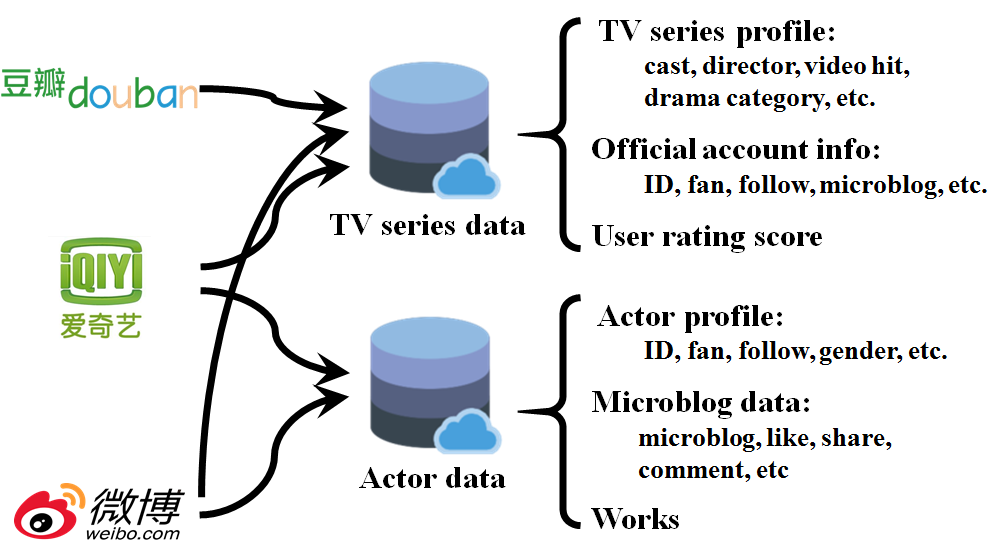
\includegraphics[height=7cm]{4}
  \caption{实验数据集}
  \label{database}
\end{figure}

\subsection{数据来源}

本文使用的实验数据,其主要的数据获取来源是爱奇艺、微博和豆瓣这三个较为流行的网站,以下对这三个网站分别进行介绍。

爱奇艺\footnote{http://www.iqiyi.com/}是国内领先的视频网站,能够提供大量电影、电视剧、综艺、动漫等视频内容供用户观看,目前已拥有超过2000万的付费用户,成为中国用户量最大的视频网站之一。为了获取更多、更全面、更准确的电视剧信息,本文通过爱奇艺网站电视剧分类下的电视剧列表获取全部的电视剧名单,并通过该列表访问各个电视剧的详情页面,从中可以获得电视剧的相关信息,包括电视剧名称、主演、导演、类型、集数、播放量、简介等信息。电视剧《欢乐颂》详情页如图~\ref{爱奇艺}所示。

\begin{figure}[h] 
  \centering
  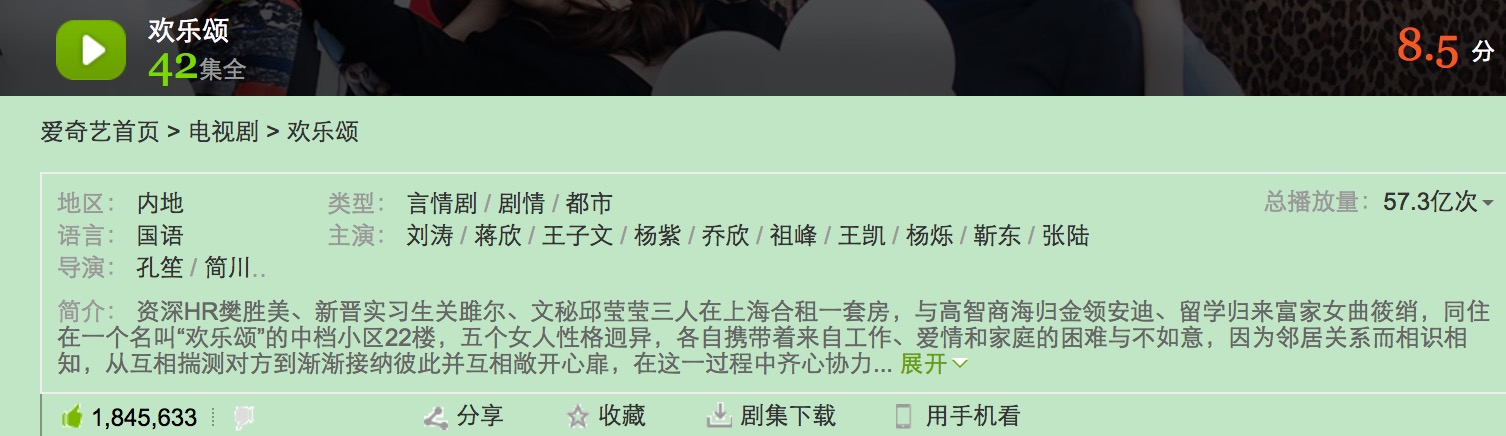
\includegraphics[height=9cm]{爱奇艺}
  \caption{电视剧《欢乐颂》的爱奇艺详情页}
  \label{爱奇艺}
\end{figure}

豆瓣\footnote{http://www.douban.com/}是一个社区网站,提供关于书籍、电影、音乐等作品的信息、评论,并且其中的所有描述和评论信息,都由用户自发提供(User-generated content, UGC),任何人都可以发表评论。在豆瓣网上较为重要的信息包括关于电影或电视剧的评分。该评分通过对各个用户对电影或电视剧的打分综合评定计算得到,能反应当前广大群众对其质量、水平的认同情况,是对电影或电视剧质量好坏的一个重要的评定参考标准。电视剧《欢乐颂》豆瓣详情页如图~\ref{欢乐颂豆瓣}所示。

\begin{figure}[h] 
  \centering
  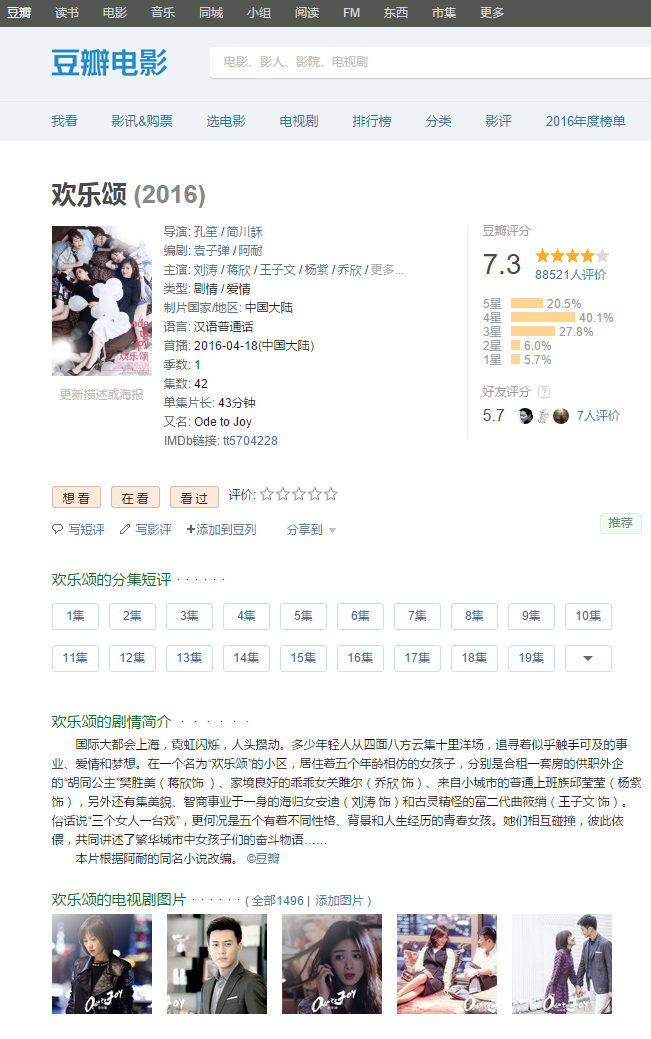
\includegraphics[height=12cm]{欢乐颂豆瓣}
  \caption{电视剧《欢乐颂》的豆瓣详情页}
  \label{欢乐颂豆瓣}
\end{figure}

微博\footnote{http://www.weibo.com/}是一个类似于Twitter的微博客网站,注册用户可以在其上发布短消息,并可以上传图片和链接视频,对于其他用户发布的微博,还可以进行评论、转发、点赞。用户可以在微博上获取新闻信息、娱乐消息,还可以进行社交互动等。现阶段,微博“占据中国微博客用户总量的57\%,以及中国微博活动总量的87\%,是中国大陆访问量最大的网站之一” \cite{微博维基}。

由于微博庞大的用户量,在微博上进行推广营销能够获得巨大的受众群,得到很好的宣传效果。因此,大部分电视剧的宣传方会在微博上创建官方微博账号,电视剧《欢乐颂》的官方微博如图~\ref{官微}所示,用来发布电视剧、演员相关的信息,比如电视剧预告、演员拍摄花絮、电视剧相关或者演员相关的推广信息等等,使得观众获得更多的关于电视剧和主演的信息和动态。

同时,大部分电视剧在微博上会有一到多个话题,以“\#话题名\#”的形式存在,且各个话题会有该话题的首页,如图~\ref{话题}所示,当用户在微博中发布微博讨论电视剧时,会在微博中加入话题名称的相关文字,其他用户就可以看到关于此话题所有用户发布的所有微博的内容。有关该话题的微博的发布数量越多,说明该话题越活跃,关注该话题的人数越多。通过话题首页,可以获得关于该话题的阅读量、话题讨论量、话题粉丝量等信息。

\begin{figure}[h]
  \centering%
  \subcaptionbox{官方微博\label{官微}}
    {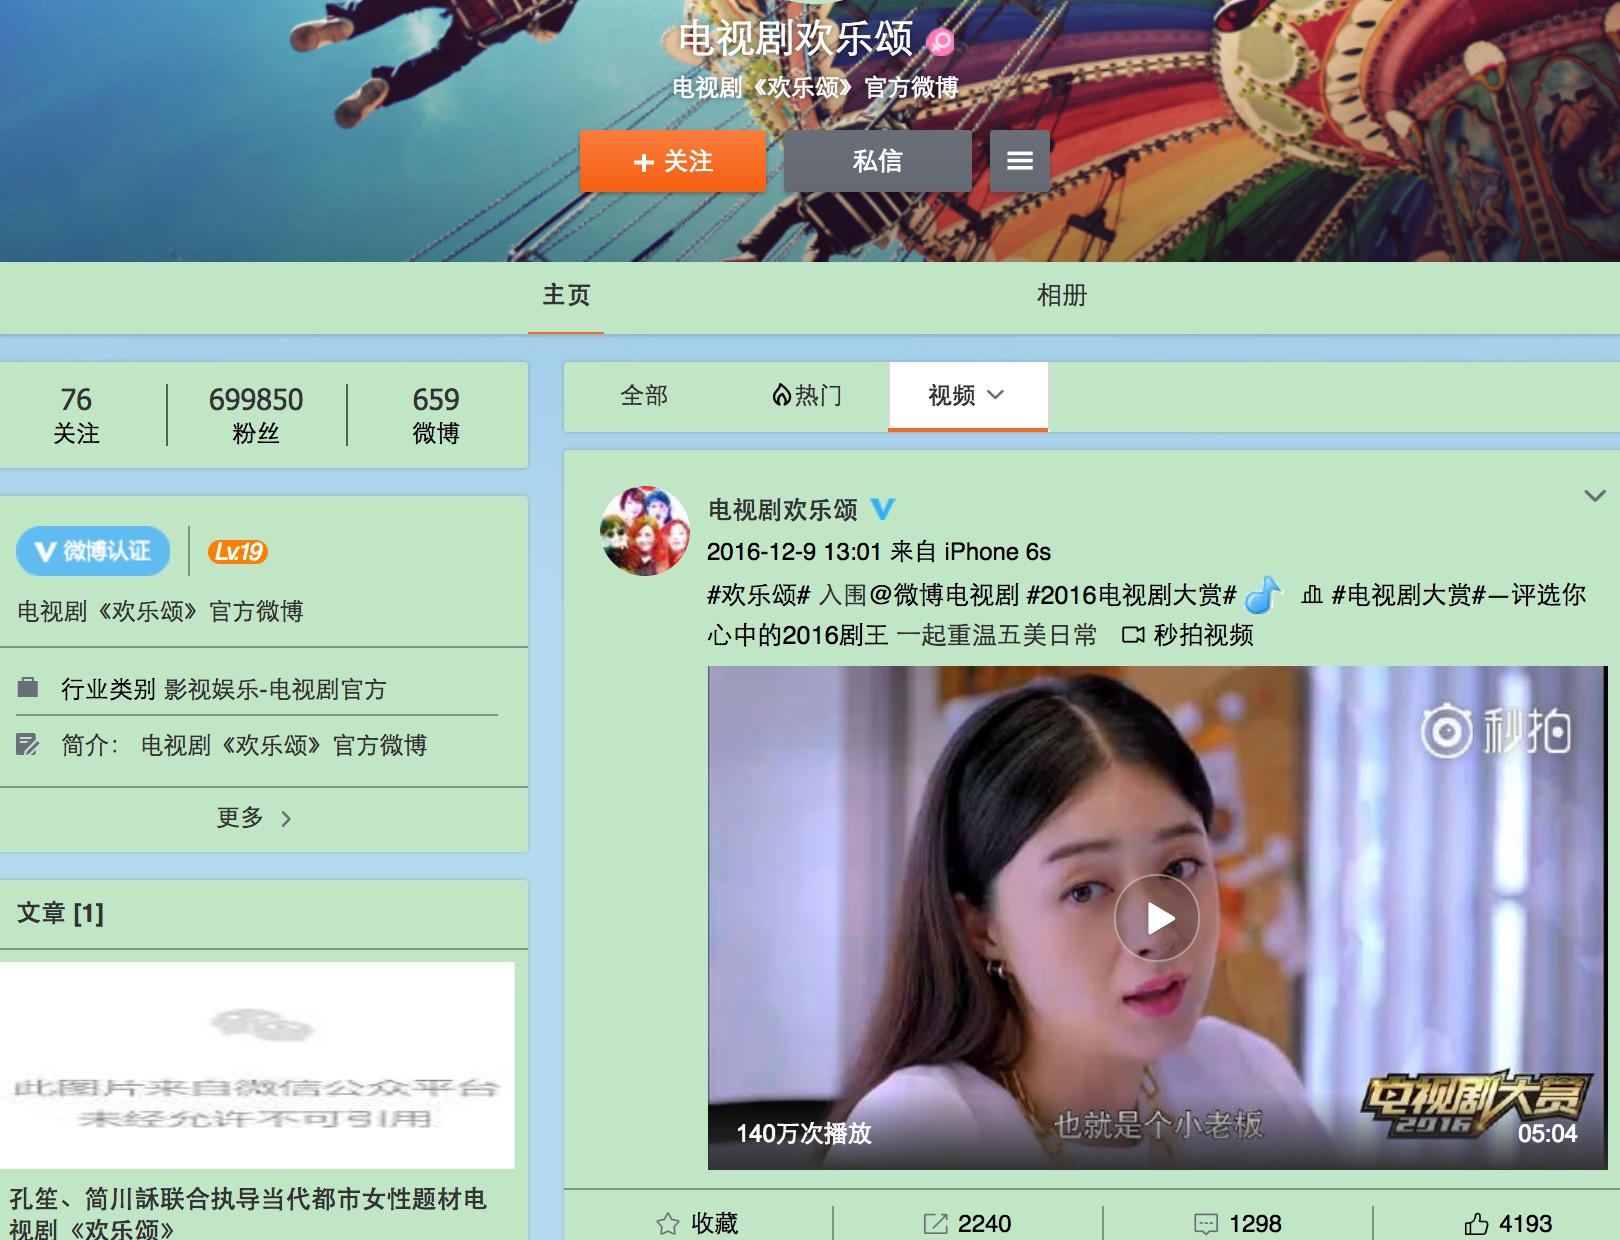
\includegraphics[height=11cm,width=7cm]{欢乐颂官微}}
  \subcaptionbox{话题主页\label{话题}}
      {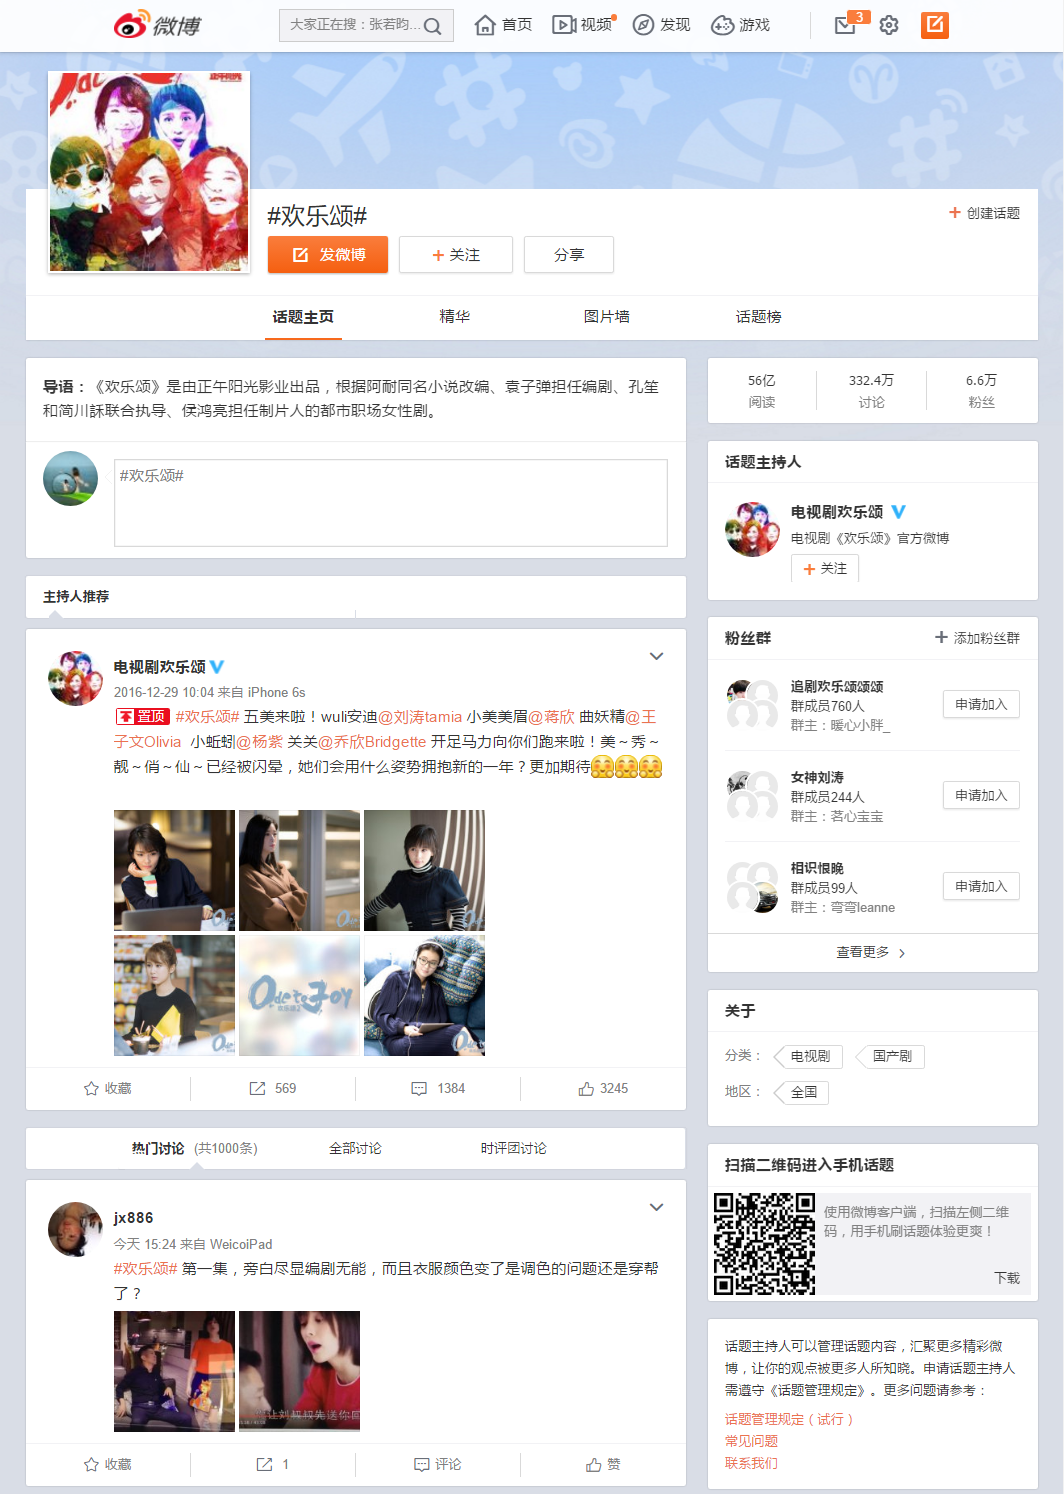
\includegraphics[height=11cm,width=7cm]{欢乐颂话题}}
  \caption{电视剧《欢乐颂》的微博详情页}
\end{figure}

另外,通过爱奇艺网站上电视剧详情页所介绍的信息,可以获得该电视剧的所有主要演员名单,将所有电视剧的所有演员汇总后,能够得到一个演员数据库。演员的详细信息可以通过微博获得,大多数演员会在微博上创建一个实名认证账户,公布关于演员自身的基本信息,并发布有关自己的生活信息、出演的影视剧信息等。如果~\ref{刘涛}所示的是电视剧《欢乐颂》的主演刘涛的微博账户。

\begin{figure}[h] 
  \centering
  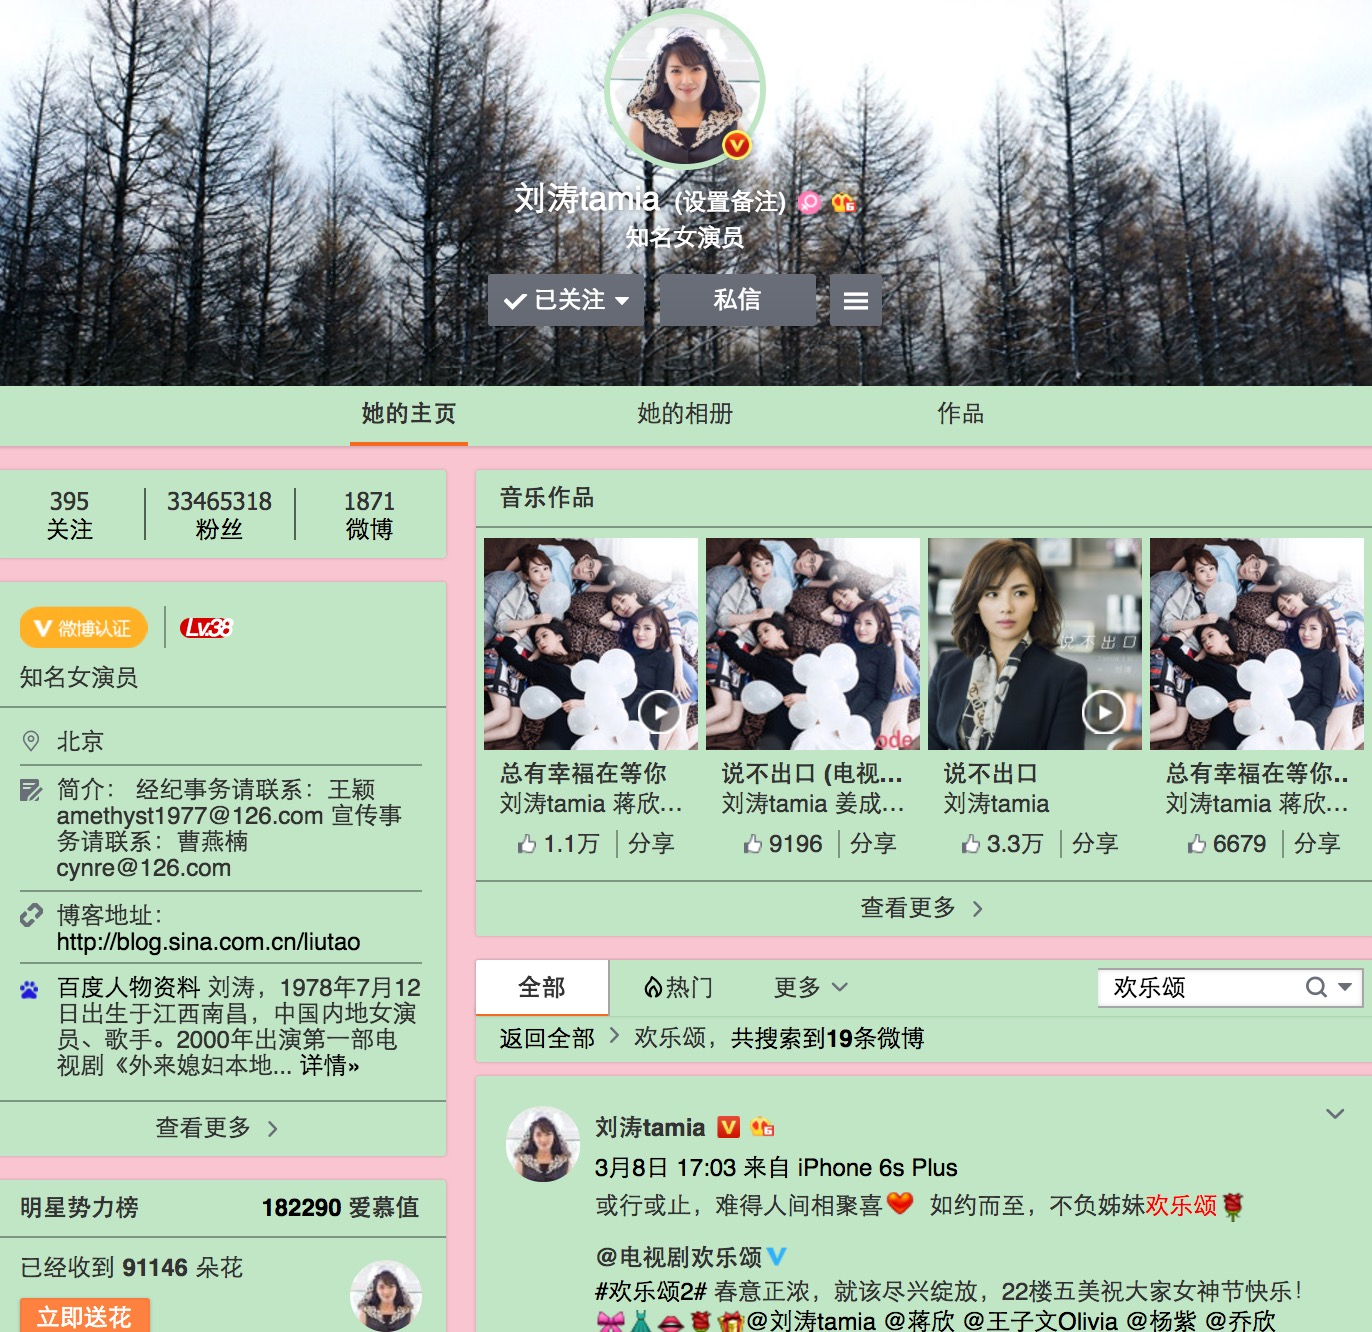
\includegraphics[height=12cm]{刘涛}
  \caption{刘涛微博主页}
  \label{刘涛}
\end{figure}

\subsection{特征提取}

本文使用的实验数据主要可以分为两部分,一是关于电视剧的信息,一是关于演员的信息,相应的数据库系统也就分为了演员数据库和电视剧数据库两部分,通过爬虫模拟登陆、模拟搜索的形式获取信息。对于电视剧信息来说,其来源主要是豆瓣和爱奇艺,而对于演员信息来说,其来源主要是微博和爱奇艺。具体数据来源结构如图~\ref{3}所示。

对于电视剧信息来说,首先利用爱奇艺爬虫通过爱奇艺电视剧首页URL,获取所有电视剧的名称和URL链接列表,然后针对名单列表内的每一部电视剧,利用爱奇艺爬虫爬取其电视剧的详情页,获取其中关于电视剧的基本信息,包括电视剧的演员、类型标签、导演、播放次数、语言、内容简介等。所有这些电视剧信息存入电视剧数据库。利用各个电视剧的演员名单,从微博中获取的这些演员的粉丝数目(具体方法见下文),求和即可得到该电视剧的演员阵容。

同时,电视剧数据库还有一部分信息来自于豆瓣网。豆瓣爬虫根据由爱奇艺网站获取的电视剧名称列表,从豆瓣搜索入口模拟搜索,访问电视剧在豆瓣网上的主页,在其主页中可以获得关于该电视剧的信息,包括该电视剧的豆瓣评分、评价人数、观众评论等。

另外,还需要在微博上获取电视剧的官方微博信息和话题信息。微博爬虫根据电视剧名称列表,获取各个电视剧在微博上官方微博的id,然后模拟访问手机端主页,获得该电视剧官方微博的基本信息,包括id、粉丝数、关注数、发布微博数等,还会提取该账号发布的所有微博信息,包括每条微博的内容、点赞数、转发数、评论数。而对于电视剧话题来说,微博爬虫根据从电视剧官方微博中出现的话题名称或者从微博搜索入口搜索电视剧,可以得到电视剧的话题名称,进而获得该电视剧话题的相关信息,包括话题阅读量、话题讨论量、话题粉丝量等。

\begin{figure}[H]
\centering
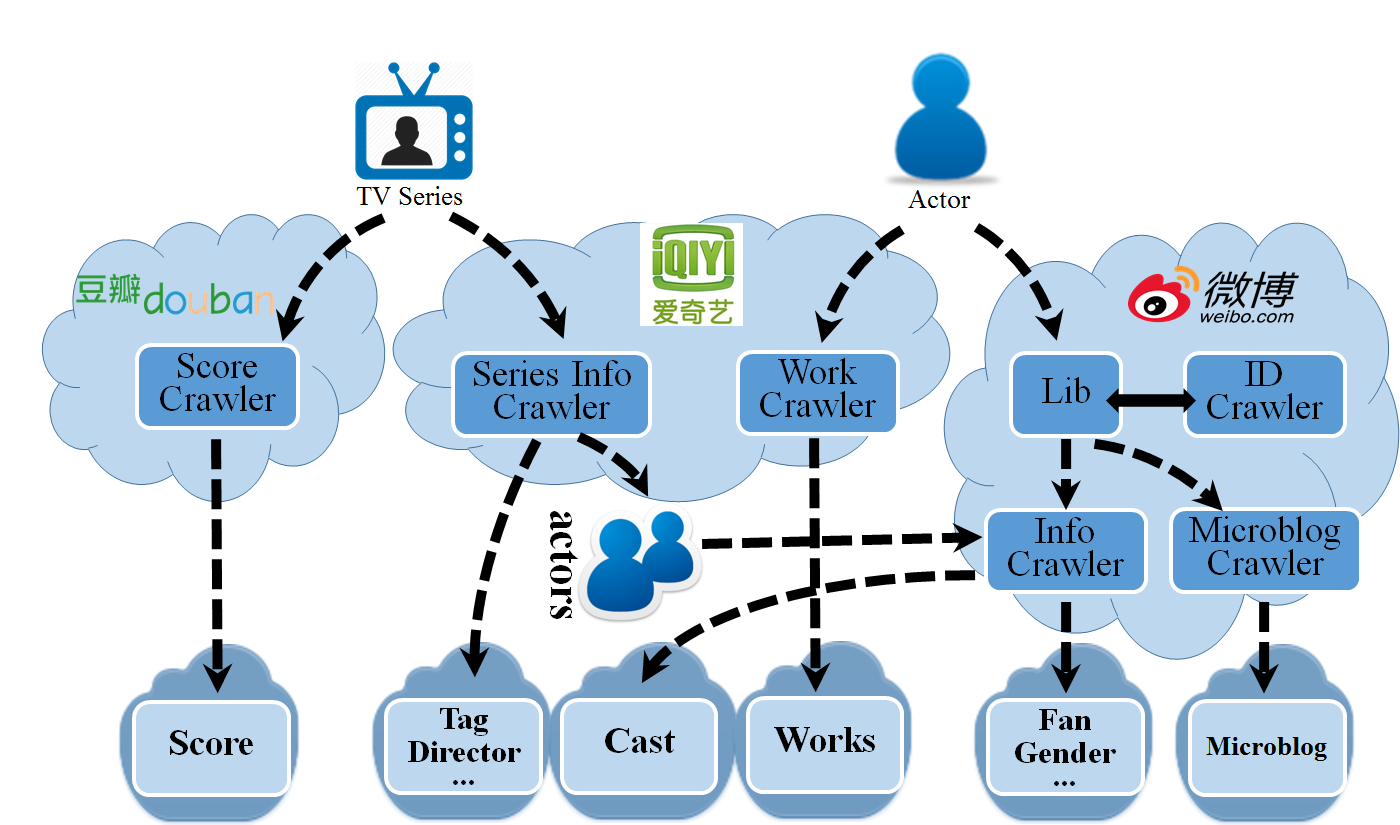
\includegraphics[height=7cm]{3}
\caption{实验数据分布结构}
\label{3}
\end{figure}

对于演员信息来说,利用爱奇艺爬虫获取电视剧的详情页后,可以从中获取该电视剧的所有主要演员名单,可以将这些主演建成一个演员数据库。利用爱奇艺爬虫爬取的电视剧的信息,可以得到每个演员出演过的作品名称和数量,反应演员在荧幕上的活跃度。

\begin{figure}[H]
\centering
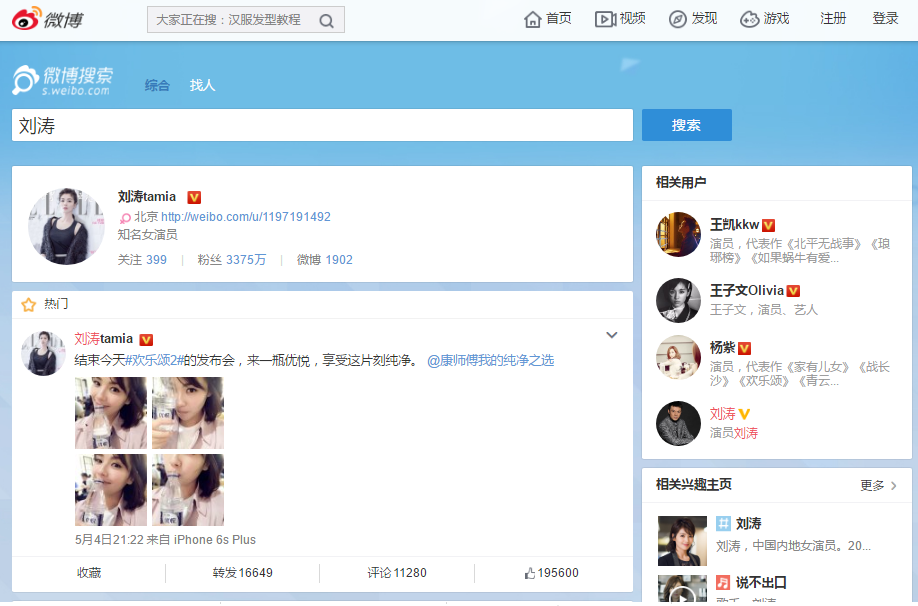
\includegraphics[height=9cm]{搜索}
\caption{从微博搜索入口查询演员微博id}
\label{搜索}
\end{figure}

然后,利用微博爬虫获取各个演员在微博上的信息。从演员名字到其在微博上id的对应采用了三种方法,第一种方法是微博爬虫根据演员名字在微博搜索入口模拟搜索,出现的第一个用户进行验证,验证方法为根据其微博认证信息中是否有演员、明星、出演等字样。在微博搜索入口查询演员刘涛的结果如图~\ref{搜索}所示:

第二种方法是从微博名人堂\footnote{http://verified.weibo.com/fame/yingshi}中得到演员在微博中的id和主页,如图~\ref{名人}所示:

\begin{figure}[!htbp]
\centering
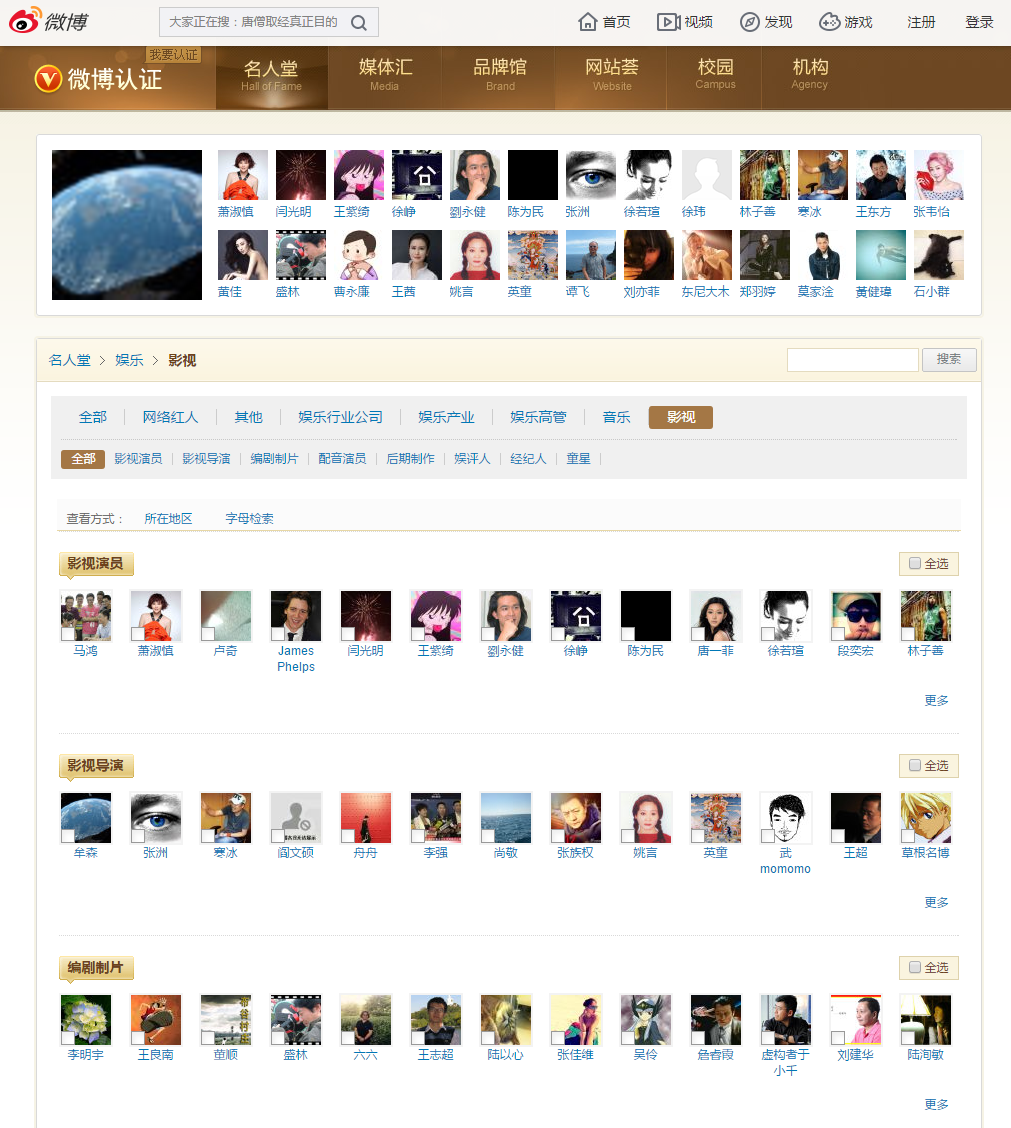
\includegraphics[height=13cm]{名人}
\caption{从微博名人堂查询演员微博id}
\label{名人}
\end{figure}

第三种方法作为补充,爬虫从百度搜索入口模拟搜索演员名字,出现的第一个认证微博用户并进行同样的验证。在百度搜索入口查询关键字“刘涛”、“微博”的结果如图~\ref{百度}所示:

\begin{figure}[!htbp]
\centering
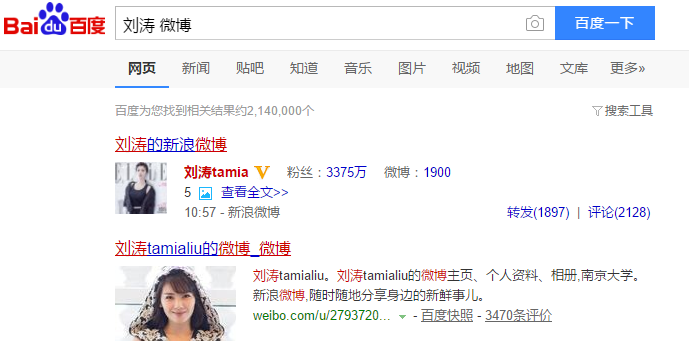
\includegraphics[height=6cm]{百度}
\caption{从百度查询演员微博id}
\label{百度}
\end{figure}

然后根据id访问演员的微博账户主页,获得演员的基本信息和发布的所有微博。其中,基本信息包括演员id、昵称、性别、描述、注册时间、粉丝数、关注数、微博数等等。同时,获得演员的id、基本信息的对应后,还进行了人工的验证筛选,以保证获得的都是对应正确的微博id。微博信息包括发布的微博内容、时间及其获得的点赞数、转发数、评论数。由于通过微博开放API在抓取微博信息时,一方面由于开发者级别低,接口访问速度慢,另一方面接口有保护隐私的考虑,在非好友状态下,能获得的信息很少。所以,我们采用了爬虫模拟登陆手机端微博的方法来爬取演员发布的所有微博信息。

电视剧的特征中,电视剧的豆瓣评分代表了群众对该电视剧质量的认同和评价;电视剧的演员阵容用该电视剧所有主演的粉丝数的总和来表示,代表了这个电视剧整体的粉丝量和可能的受关注度,越多名人参与到同一部电视剧中,这个电视剧越容易流行。微博自身的特征是由发布微博的演员决定的,包括时间、日期和内容,这是我们研究的主要内容。发布微博的演员的特征中,粉丝数代表该演员在微博中的影响力,当两个不同粉丝量的演员发布同一条微博时,粉丝量大的演员发布的微博会被更多的人看到,也就更容易达到更好的推广作用;男演员和女演员的行为本身有差异,其粉丝男女构成也有差异,相应的粉丝行为和对推广微博的反馈行为也会有差异;演员的作品数代表该演员在荧屏上的活跃程度,演员出演的电视剧越多,越容易被观众记住也越有名。

各个网站的爬虫运行在服务器端。对于电视剧信息,其获取时间从2013年1月到2016年12月31日,期间每天爱奇艺电视剧列表会有3000部电视剧,我们的爬虫会对这些电视剧的信息进行爬取。对演员信息,我们获得了8508个对应到微博id的演员,并获得了他们的基本信息和发布的所有微博信息,微博爬虫每隔三个月从微博上对演员信息增量爬取。下文的研究因操作时间不同,选取的电视剧有所差异,主体的研究数据是首播时间在2016年1月1日到2016年12月31日的电视剧,共313部,包含了1121个不同的演员及其在这段时间内发布的114767条微博。

\section{测量分析}

本节针对获取到的数据,进行了初步的分析和测量,并从中挖掘数据特征和规律。基于粉丝参与度,提出微博影响力指数来衡量每一条微博的影响力。分析了微博影响力与话题热度的相关性。还分析了演员在微博中对电视剧的推广模式,还发现了一些推广规律。

\subsection{微博影响力与话题热度}

\textbf{(1) 微博影响力。}
为了衡量一条微博的影响力,我们采用粉丝参与度作为评判标准,包括这条微博的转发数、评论数和点赞数,因为这些数据能反应看到并参与到电视剧推广中的用户数量。经过统计,在数据库中所有演员的所有微博的转发数、评论数、点赞数的比例是${1: 1.86: 4.66}$。为了使这三项评判指标具有相同重要程度,因此赋予其权重比为${4.66: 2.51: 1}$,从中也能反应出转发、评论和点赞能带来的不同影响力。转发推广微博能使转发人的粉丝也看到,用户的参与感非常强,转发的人多了就具有滚雪球效应,能扩大宣传效果,因此其权重最大。用户通过评论推广微博参与到推广中,评论越多也越容易使该演员上微博热门,但评论并没有扩大用户群,所以用户参与感和影响力不如转发大。相比于转发和评论,用户点赞既不会扩大用户群也不需要输入文字,其用户参与感最弱,所以权重最小。定义微博影响力公式如下:

\begin{equation}P_i^j = 4.66 * W_p^i + 2.51 * W_v^i + W_a^i\end{equation}

其中,$P_i^j$ 表示与电视剧$j$相关的微博$i$的影响力,$W_p^i$, $W_v^i$和$W_a^i$分别表示微博$i$的粉丝转发数、评论数和点赞数。

那么对一部电视剧带来说,微博影响力是其所有主演发布的推广微博的影响力之和:

\begin{equation}T_j = \sum_{i=1}^n P_i^j\end{equation}

其中$T_j$表示电视剧$j$所有主演的推广微博影响力之和,$n$为电视剧主演发布微博的数量。

\textbf{(2) 电视剧微博话题热度。}
我们研究的每部电视剧,在微博中都有对应的微博话题。每个微博话题都有相应的阅读量和讨论量,其中阅读量表示该话题的用户阅读数目,讨论量表示用户发布的带该话题名称的微博数目。在电视剧上映前和上映中进行宣传时,宣传方都会以“\#话题名\#”的形式发布微博。话题讨论量和阅读量越多,表明越多的用户参与到该话题讨论中,越容易成为热门话题,进而达到更好的宣传效果。用户带话题名发布微博,会增加微博话题讨论量,使其粉丝看到该微博,提高微博话题阅读量。也就是说微博话题阅读量是话题讨论和宣传效果的体现,代表了该电视剧微博话题覆盖到的人数,是其热度的体现。因此我们选用电视剧的微博话题阅读量来衡量电视剧在微博中的话题热度:

\begin{equation}H_j = R_j\end{equation}

其中$H_j$表示电视剧$j$的微博话题热度,$R_j$表示微博话题的阅读量。

\textbf{(3) 微博影响力与话题热度的相关性。}
为检验电视剧微博影响力与话题热度的相关性,我们选用皮尔森相关系数(Pearson correlation coefficient)和最大信息系数(Maximal Information Coefficient, MIC)来进行检验。皮尔森相关系数可以反映出两个变量之间的线性相关程度,系数的变化范围为-1到1。系数值为1意味着变量X和Y呈完全正相关关系,Y随X增加而增加。系数值为-1意味着X和Y呈完全负相关关系,Y随X增大而减小。系数值为0意味着两个变量间没有线性关系。MIC是专门用于快速探索多维数据集的双变量依赖关系的度量。MIC是基于信息的非参数探索(MINE)统计方法系列的一部分,MINE不仅可用于识别数据集中的重要关系,还可用于表征数据集。MIC可以分析变量之间的广泛关系,而不限定于特定的函数类型\cite{10}。

经过统计,电视剧的微博影响力与最终话题热度高度相关,两者之间相关性如表~\ref{rel}所示。因此,可以将微博影响力作为微博话题热度的评判标准,即在判断推广微博带来的营销效果时,推广电视剧的微博影响力大则说明该电视剧话题热度高。电视剧话题演化的和微博影响力的动态数据也验证了二者之间的相关性。以电视剧《欢乐颂》为例,电视剧微博话题热度与微博影响力每日变化如~\ref{huanl}图所示,从图中可以看出,二者趋势和形状几乎一致。

\begin{table}[h]
\centering
\caption{微博影响力与话题热度的相关性计算结果}
\label{rel}
\begin{tabular}{|c|c|c|c|} \hline
variable x&varible y&PCC&MIC\\ \hline
influence&hotness&0.697&0.356\\
\hline\end{tabular}
\end{table}

\begin{figure}[!htbp]
\centering

\includegraphics[width=11cm]{1}
\caption{《欢乐颂》微博话题热度与微博影响力每日变化}
\label{huanl}
\end{figure}

\subsection{推广模式}

演员在微博上发布的推广电视剧的微博可以按照推广周期、推广时间和互动模式进行分类,可以得到这几种推广模式下的多种推广策略,进而可以利用算法对各种推广策略进行评估。

\textbf{(1) 推广周期。}
演员对电视剧的推广周期主要可分为三个阶段,一是电视剧的筹备、拍摄阶段,二是电视剧首播阶段即第一集播出前后,三是首播之后的阶段。以电视剧《杉杉来了》为例,其主演发布微博的数量统计如图~\ref{shan}所示。演员在电视剧拍摄期间会分享一些电视剧拍摄地、拍摄进度、角色和剧情相关信息等内容,这些微博不但可以让粉丝对演员的动态有所了解,还可以让观众提前了解电视剧相关信息,引起粉丝的兴趣和期待,起到提前宣传的作用。在第一集播放的前后几天是演员和电视剧官方宣传的高峰期,演员会发布微博进行大力度推广,我们将电视剧首集首播日前后5天定义为电视剧的首播阶段。统计发现虽然有些演员在微博中不活跃,但是仍然会在首播前后,发布微博进行推广宣传。首播阶段是影响收视率的关键时间,在这个时期演员推广可以提醒和号召粉丝观看这部电视剧,促进提高话题热度和收视率。首播之后,演员还会继续进行微博推广,发布微博传递信息或者与粉丝互动,能在维持现有观众继续观看后续剧集的同时,吸引更多观众参与话题讨论并提高电视剧收视率。除此之外,当电视剧登陆其他电视台开播时,演员也会发布微博进行推广。因此,从推广周期来看,演员推广微博时期分为三类,分别为筹备阶段、首播阶段和首播后阶段。

\begin{figure}[!htp]
\centering
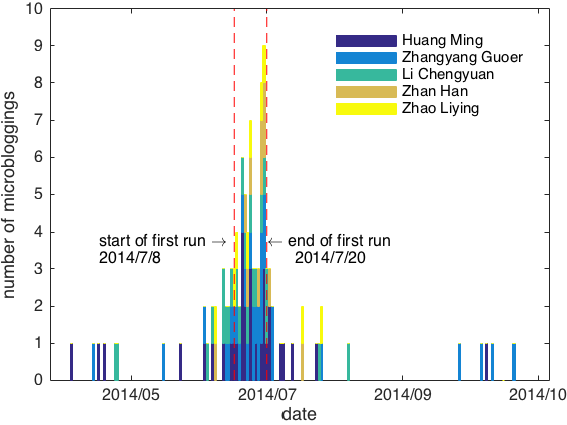
\includegraphics[width=9cm]{period}
\caption{演员发布微博的数量统计}
\label{shan}
\end{figure}

\textbf{(2) 推广时间。}
在一天中不同时间发布推广微博,由于用户使用习惯的差异,被用户看到的时长和概率不同,也就会达到不同的推广效果。比如同一条推广微博,在用户浏览微博高峰和上班时间发布,肯定会获得不同的参与度。在一天中,午饭前、晚饭前及晚上通常都是用户浏览微博的高峰时段。图~\ref{time}显示了演员发布微博时间的分布情况,同时也包括演员在电视剧上映前和上映后的数目差异。在本文中,我们想知道演员在不同时间段发布微博,哪个时间段会带来更好的推广效果,因此,我们将演员发布的微博根据发布时间分成三类,分别是上午(1时至12时),下午(12时至18时),晚上(18时至次日1时)。

\begin{figure}[!htbp]
\centering
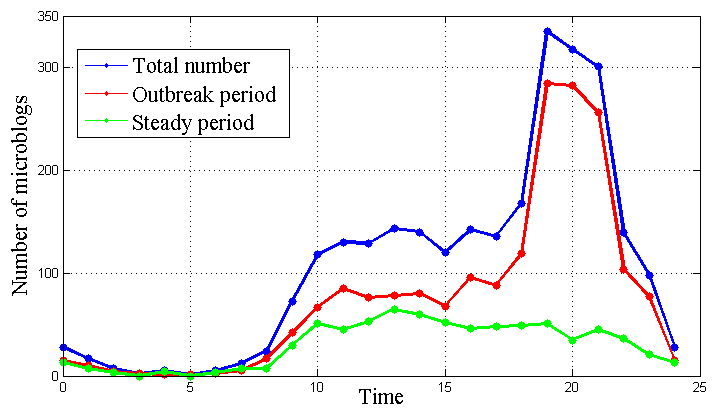
\includegraphics[width=10cm]{time}
\caption{演员发布微博数量在一天当中的分布图}
\label{time}
\end{figure}

\textbf{(3) 互动模式。}
在微博上推广电视剧过程中,演员会与其他主演、粉丝、电视剧官方微博等有很多交互行为来增加用户的参与度,促进电视剧的推广。图~\ref{inter2}展示了电视剧《欢乐颂》推广过程中出现的互动关系。图中每个节点表示一个演员或者官方微博账号,节点大小代表了与其他账号互动的数目,发过的微博中与其他账号互动越多,节点大小越大。有向箭头表明了互动的方向,边的粗细代表互动的频率,频率越高边越粗。
\begin{figure}[!htbp]
\centering
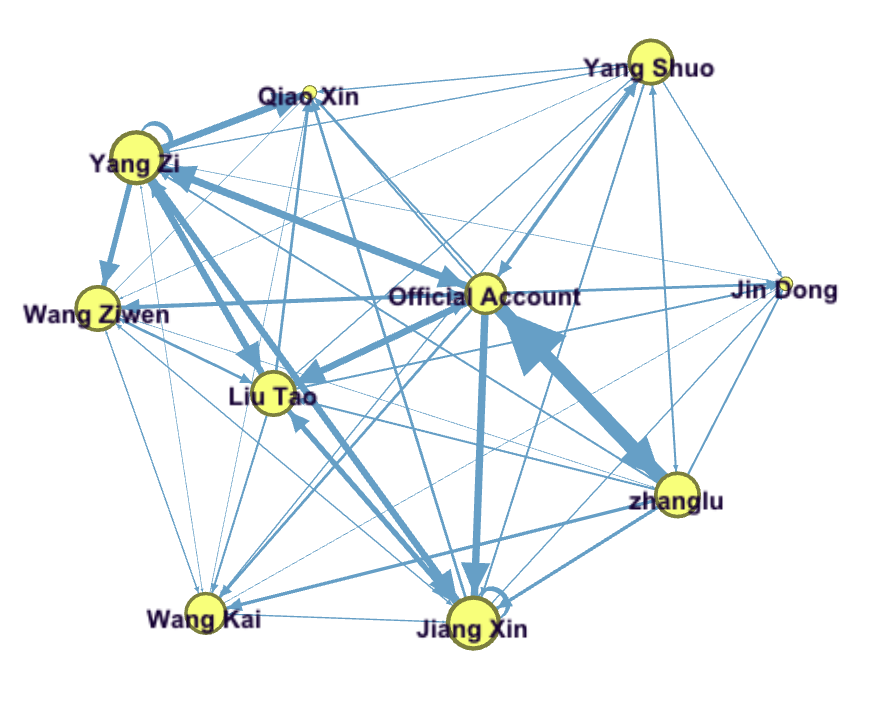
\includegraphics[width=9cm]{interaction}
\caption{电视剧《欢乐颂》的微博互动关系}
\label{inter2}
\end{figure}

一条微博可以使演员间、演员与官方微博间、演员与粉丝间建立互动关系,图~\ref{inter}中表示了一条微博的传播情况,图中黄色点是该电视剧的主演,每个点是一个微博用户,每条边是一个转发关系。

演员发布推广微博时有四种互动模式:
\begin{itemize}

\begin{figure}[H]
\centering
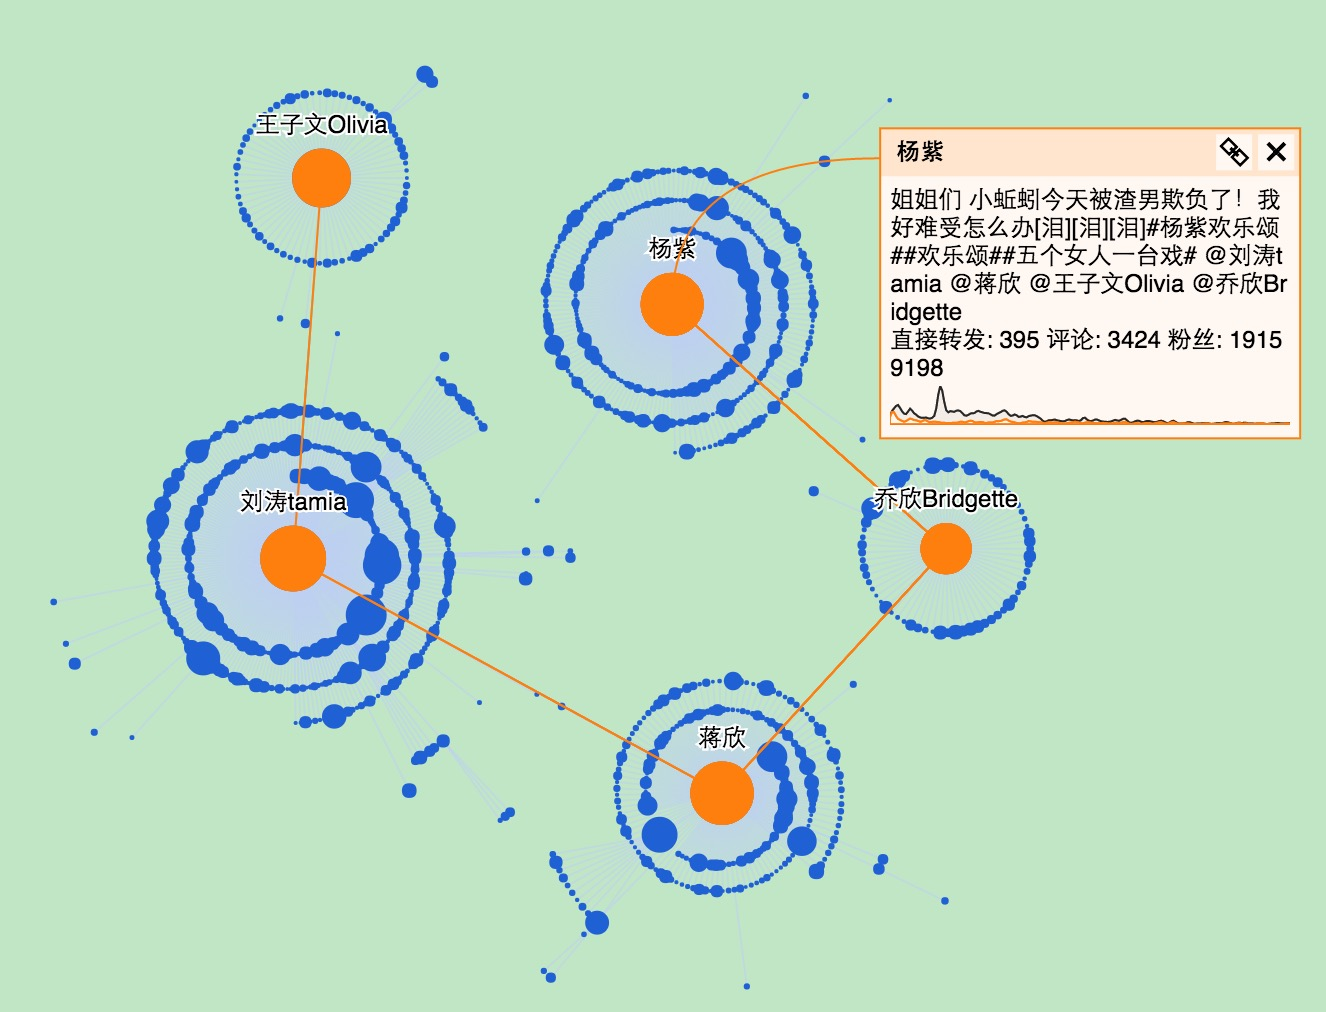
\includegraphics[height=11cm]{微博互动}
\caption{微博互动关系}
\label{inter}
\end{figure}

\item[(1)]与电视剧其他主演互动。演员会转发其他主演微博,或者发布微博“@”其他主演,在微博中与其他主演进行交流。主演间互动一方面会增加 微博话题性,另一方面也会结合多方粉丝,扩大推广效应。

\item[(2)]与官方微博互动。经过统计发现,一种常见的推广模式是,官方微博作为源头,发布推广微博,并在微博中“@”主演,主演将会转发这条微博,提升官方微博推广的影响力。我们用累计分布图来分析演员响应官方微博的时间概率分布。以电视剧《欢乐颂》为例,78\%的主演的响应时间在2小时以下,如图~\ref{fig}(a)。统计发现,对所有电视剧而言如图~\ref{fig}(b),80\%的主演的响应时间都会在12小时以下。

\begin{figure}[h]
  \centering%
  \subcaptionbox{电视剧《欢乐颂》}
    {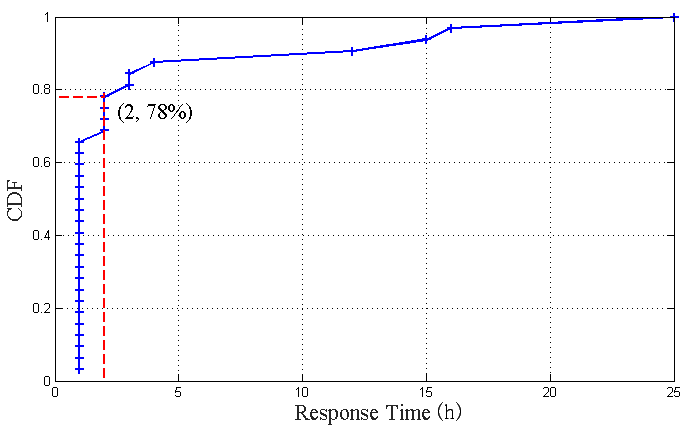
\includegraphics[width=7cm]{53}}
  \subcaptionbox{全部电视剧}
      {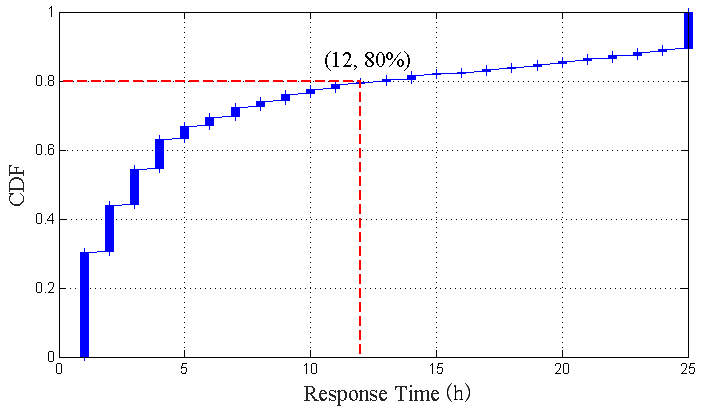
\includegraphics[width=7.4cm]{52}}
  \caption{演员响应官方微博的时间概率分布}
  \label{fig}
\end{figure}

\item[(3)]原创非互动微博。此类微博由演员原创,虽然不包含与其他人的互动,但通过表达针对电视剧剧情或者人物的感想和看法,更好的表达演员的情感和想法,更能够吸引粉丝注意和参与。

\item[(4)]其他互动模式。与除演员、官方微博外的其他微博用户互动称为其他互动模式,包括演员转发视频网站官方微博的微博、转发粉丝微博、转发宣传媒体微博等。

\end{itemize}

图~\ref{inter3}显示了所有演员发布的微博中,以上四种模式所占的比例。其中图~\ref{inter3}(a)为整个电视剧周期中的四种模式的比例,图~\ref{inter3}(b)为电视剧首映前的比例,图~\ref{inter3}(c)为电视剧首映后的比例。

\begin{figure}[!htbp]
\centering
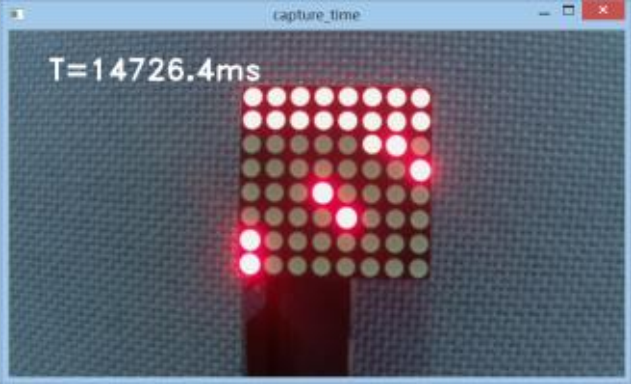
\includegraphics[width=11cm]{6}
\caption{互动模式比例分布}
\label{inter3}
\end{figure}

\textbf{(4) 推广模式与话题热度。}
为验证各种推广模式与话题热度的相关性,我们用皮尔森相关系数PCC和最大信息系数MIC\cite{10}来检验。通过两种检测方法可以表明各个推广模式与话题阅读量具有较强的相关性,因此接下来我们就可以评估各个推广模式下的推广策略与话题热度的因果性。

\begin{table}[!htbp]
\centering
\caption{各种推广模式与话题热度的相关性}
\begin{tabular}{|c|c|c|c|} \hline
\multicolumn{2}{|c|}{推广模式}&PCC&MIC\\ \hline
\multirow{3}{*}{推广周期} & 筹备阶段&0.389&0.284\\% \hline
&首播阶段&0.515&0.342\\% \hline
&首播后阶段&0.813&0.399\\ \hline
\multirow{3}{*}{推广时间} &早上&0.239&0.306\\% \hline
&中午&0.542&0.407\\% \hline
&晚上&0.856&0.340\\ \hline
\multirow{3}{*}{互动模式} &主演互动&0.390&0.292\\% \hline
&与官微互动&0.745&0.356\\% \hline
&原创&0.600&0.297\\ 
&其他互动&0.630&0.349\\ 
\hline\end{tabular}
\end{table}

\section{本章小结}

本节主要介绍了数据集的来源、获取方法和主要内容。然后对这些数据进行整理、分析和挖掘,做一些相关测量,挖掘出一些规律。同时识别出演员在微博上发布推广微博的推广模式,对每一个推广模式进行分析,并得到其下的各种推广策略。




















































